\section{Simplified \SLCO}
\label{sec:SLCO:simplified_slco}
The \SLCO metamodel discussed in Section~\ref{sec:slco:metamodel} and the communication diagrams shown in the rest of this chapter allow a transition to have multiple statements.
When a transition is made from one state to another, the statements that are part of this transition are executed one by one.
We have already mentioned in Section~\ref{sec:slco:metamodel} that the execution of statements related to a given transition can be interleaved by the execution of statements related to a transition of a concurrent state machine.
In fact, after executing one of the statements related to a transition, an implicit intermediate state is reached.
In some cases, it is convenient to make all these implicit intermediate states explicit.
Figure~\ref{fig:slco:SLCOExampleSMSMinimized} show simplified versions of the state machines of Figure~\ref{fig:slco:SLCOExampleSMS}.
In these simplified state machines, each transition has at most one statement.
Because of this, the state machines have no implicit intermediate states.

\begin{figure}[hbt]
  \centering
  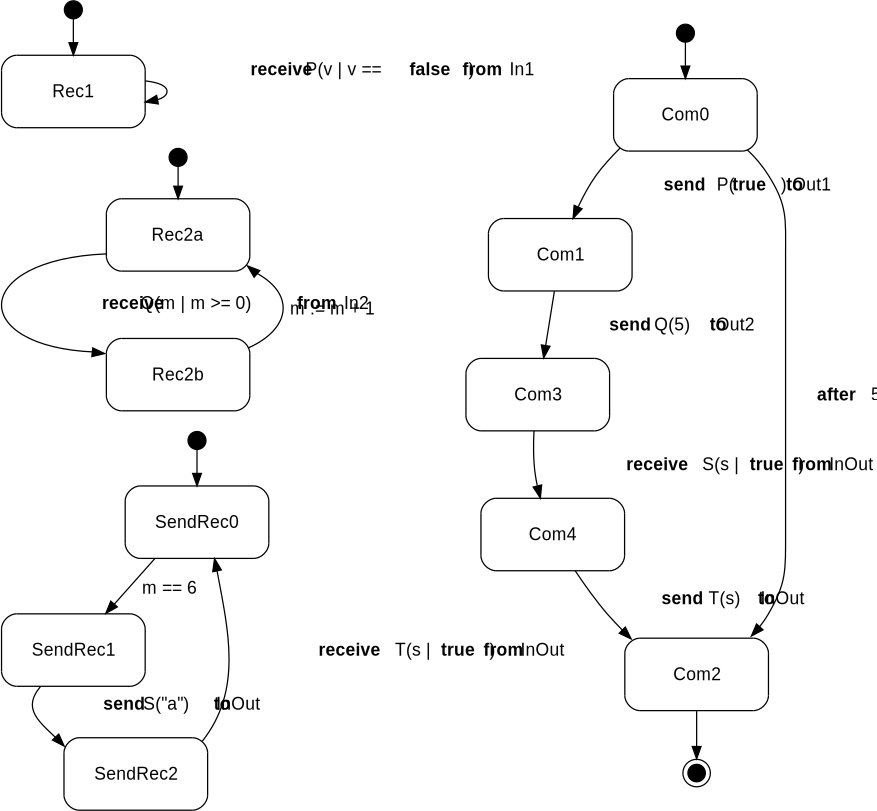
\includegraphics[scale=0.45]{slco/figs/CoreWithTimeMinimized/Behavior_CoreWithTimeMinimized}
  \caption{State machines of the simplified version of the \SLCO model of Figure~\ref{fig:slco:SLCOExampleSMS}}
  \label{fig:slco:SLCOExampleSMSMinimized}
\end{figure}

Additionally, the simplified state machines only use the general form of conditional signal reception.
To replace the shorthand notation originally used by state machine~\SLCOStateMachine{Rec1}, an auxiliary variable~\SLCOVariable{v} is introduced.
Furthermore, the expression~\SLCOTrue is added as a condition to the signal reception statements of state machines~\SLCOStateMachine{SendRec} and~\SLCOStateMachine{Com}.

The version of \SLCO that allows only these simplified state machines is used in Chapter~\ref{chap:prototype-semantics}, which discusses the process of prototyping the semantics of the language.
The formal semantics of \SLCO discussed in Appendix~\ref{ap:sos-slco} and applied in Chapter~\ref{chap:reusable-correct-transformations} is also based on this simplified version of \SLCO. 